\begin{minipage}[b]{\textwidth}

\centering
\normalsize

\tikzset{every picture/.style={line width=0.75pt}} %set default line width to 0.75pt        

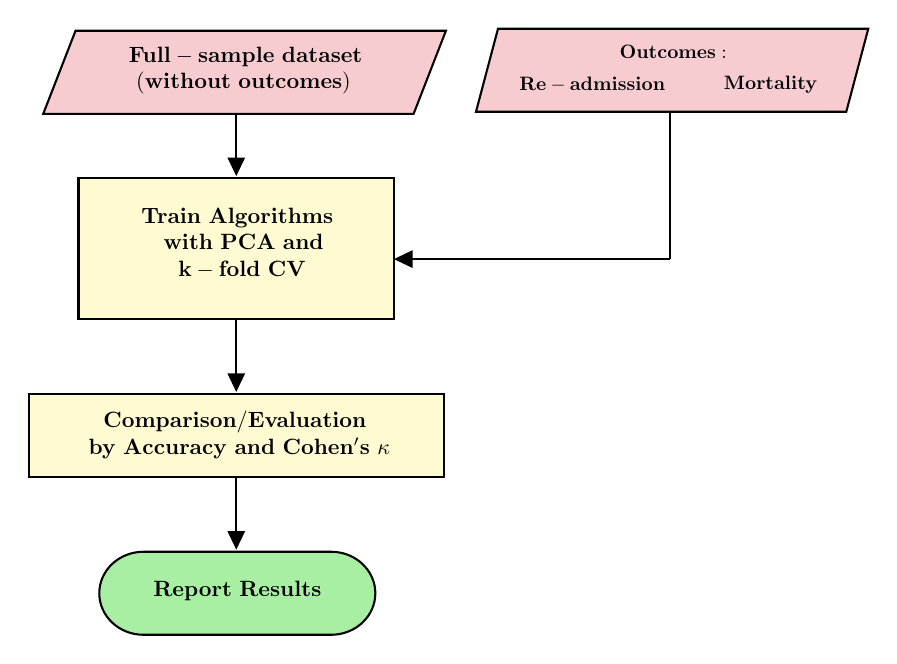
\begin{tikzpicture}[x=0.75pt,y=0.75pt,yscale=-1,xscale=1]
%uncomment if require: \path (0,401); %set diagram left start at 0, and has height of 401

%Shape: Parallelogram [id:dp1345085496641345] 
\draw  [fill={rgb, 255:red, 208; green, 2; blue, 27 }  ,fill opacity=0.2 ] (214.05,27) -- (392.5,27) -- (376.95,67) -- (198.5,67) -- cycle ;
%Straight Lines [id:da2529734460759472] 
\draw    (291.5,67) -- (291.5,95) ;
\draw [shift={(291.5,97)}, rotate = 270] [fill={rgb, 255:red, 0; green, 0; blue, 0 }  ][line width=0.75]  [draw opacity=0] (8.93,-4.29) -- (0,0) -- (8.93,4.29) -- cycle    ;

%Shape: Rectangle [id:dp8537246297754715] 
\draw  [fill={rgb, 255:red, 248; green, 231; blue, 28 }  ,fill opacity=0.2 ] (215.5,98) -- (367.5,98) -- (367.5,166) -- (215.5,166) -- cycle ;
%Shape: Parallelogram [id:dp3026993474655866] 
\draw  [fill={rgb, 255:red, 208; green, 2; blue, 27 }  ,fill opacity=0.2 ] (417.6,26) -- (596,26) -- (585.4,66) -- (407,66) -- cycle ;
%Straight Lines [id:da11621318058538299] 
\draw    (500.5,66) -- (500.5,137) ;


%Straight Lines [id:da5046262970656357] 
\draw    (369.5,137) -- (500.5,137) ;

\draw [shift={(367.5,137)}, rotate = 0] [fill={rgb, 255:red, 0; green, 0; blue, 0 }  ][line width=0.75]  [draw opacity=0] (8.93,-4.29) -- (0,0) -- (8.93,4.29) -- cycle    ;
%Shape: Rectangle [id:dp6205627904748299] 
\draw  [fill={rgb, 255:red, 248; green, 231; blue, 28 }  ,fill opacity=0.2 ] (191.5,202) -- (391.5,202) -- (391.5,242) -- (191.5,242) -- cycle ;
%Straight Lines [id:da7285903815225594] 
\draw    (291.5,166) -- (291.5,199) ;
\draw [shift={(291.5,201)}, rotate = 270] [fill={rgb, 255:red, 0; green, 0; blue, 0 }  ][line width=0.75]  [draw opacity=0] (8.93,-4.29) -- (0,0) -- (8.93,4.29) -- cycle    ;

%Straight Lines [id:da5366229358958934] 
\draw    (291.5,242) -- (291.5,275) ;
\draw [shift={(291.5,277)}, rotate = 270] [fill={rgb, 255:red, 0; green, 0; blue, 0 }  ][line width=0.75]  [draw opacity=0] (8.93,-4.29) -- (0,0) -- (8.93,4.29) -- cycle    ;

%Flowchart: Terminator [id:dp45661416532888843] 
\draw  [fill={rgb, 255:red, 139; green, 233; blue, 134 }  ,fill opacity=0.75 ] (246.78,278) -- (337.22,278) .. controls (348.97,278) and (358.5,286.95) .. (358.5,298) .. controls (358.5,309.05) and (348.97,318) .. (337.22,318) -- (246.78,318) .. controls (235.03,318) and (225.5,309.05) .. (225.5,298) .. controls (225.5,286.95) and (235.03,278) .. (246.78,278) -- cycle ;

% Text Node
\draw (296,46) node [scale=0.8]  {$ \begin{array}{l}
\mathbf{Full-sample\ dataset}\\
\mathbf{\ ( without\ outcomes)}
\end{array}$};
% Text Node
\draw (292,130) node [scale=0.8]  {$ \begin{array}{l}
\mathbf{Train\ Algorithms}\\
\ \ \ \mathbf{with\ PCA\ and\ }\\
\ \ \ \ \ \mathbf{k-fold\ CV}
\end{array}$};
% Text Node
\draw (463,53) node [scale=0.7]  {$\mathbf{Re-admission}$};
% Text Node
\draw (549,53) node [scale=0.7]  {$\mathbf{Mortality}$};
% Text Node
\draw (502,37) node [scale=0.7]  {$\mathbf{Outcomes:}$};
% Text Node
\draw (293,222) node [scale=0.8]  {$ \begin{array}{l}
\ \ \mathbf{Comparison/Evaluation}\\
\mathbf{by\ Accuracy\ and\ Cohen's\ \kappa }
\end{array}$};
% Text Node
\draw (292,297) node [scale=0.8]  {$\mathbf{Report\ Results}$};

\end{tikzpicture}


\end{minipage}